\documentclass[12pt,a4paper]{article}
\usepackage[utf8]{inputenc}
\usepackage[T1]{fontenc}
\usepackage[italian]{babel}
\usepackage{graphicx}
\usepackage{amsmath}
\usepackage{amssymb}
\usepackage{geometry}
\geometry{margin=2.5cm}

\title{Esperienza 0}
\author{Gioele Antognoni, Marco Paoletti, Giovanni Zugarini}
\date{}

\begin{document}

\maketitle

\section*{Obiettivi dell'esperienza}

\begin{enumerate}
    \item Realizzare un piccolo programma Python per registrare e ri-ascoltare un segnale audio dalla scheda audio del PC.
    \item Realizzare un piccolo programma Python che plotti un semplice grafico.
    \item Realizzare un programma Python che registri un segnale audio, lo faccia ri-ascoltare e ne plotti la waveform.
    \item Realizzare un programma Python per trasferire stringhe di testo via socket.
    \item Realizzare un programma Python per trasferire un array via socket.
    \item Realizzare un programma Python che registri un segnale audio (definire un protocollo!), lo trasferisca via socket e il ricevente lo faccia ri-ascoltare e ne plotti la waveform.
\end{enumerate}

A seguire nel documento saranno riportate le informazioni, a nostro avviso, più importanti per motivare e comprendere i risultati ottenuti.

\section{Metodologia}

\subsection{Audio WhatsApp}

Per completare la prima fase dell'esperienza avevamo la necessità di accedere, tramite Python, ai microfoni e agli altoparlanti del computer; abbiamo quindi optato per l'utilizzo della libreria \textit{soundcard}. Inizialmente abbiamo visualizzato tutti i canali audio di input e output del nostro dispositivo, scegliendo nello specifico con quale microfono registrare il segnale e con quale altoparlante riascoltarlo. La libreria permette di impostare sia la frequenza di campionamento (\textit{samplerate}) sia il numero totale di campioni (\textit{numframes}). Nel nostro caso abbiamo impostato:
\begin{itemize}
    \item \textit{samplerate} = 48000 Hz
    \item \textit{numframes} = 480000
\end{itemize}

Il microfono selezionato (\textit{<Microphone Gruppo microfoni (*<Tecnologia Intel® Smart Sound per microfoni digitali) (2 channels)>}) dispone di 2 canali. Di conseguenza, l'output della registrazione è un array contenente \textit{numframes} coppie di valori, corrispondenti alle variazioni di pressione registrate da ciascun canale, legate all'ampiezza delle onde sonore ricevute. I dati attesi sono adimensionali e compresi nell'intervallo $[-1, 1]$, in quanto rappresentano l'ampiezza dell'onda rilevata rispetto alla massima pressione convertibile dal nostro convertitore analogico-digitale (\textit{ADC}).

Per il riascolto della registrazione abbiamo utilizzato l'altoparlante di default (\textit{<Speaker Speaker (Realtek(R) Audio) (2 channels)>}) a 2 canali, specificando la frequenza di riproduzione del segnale. Questa funzionalità permette di riprodurre l'audio anche a velocità diverse rispetto a quella originale. Nel nostro esperimento abbiamo testato le velocità 1x, 1.5x, 2x e 4x, moltiplicando il parametro \textit{samplerate} per il corrispondente fattore. Abbiamo riscontrato che, all'aumentare della frequenza di riproduzione, il suono diventa progressivamente più acuto.

Infine, risulta utile normalizzare i dati della registrazione dividendo l'intero array per il suo valore massimo assoluto: in questo modo si porta il picco del segnale al limite massimo consentito dalla scala digitale $(1.0)$, garantendo il massimo volume di riproduzione senza incorrere in distorsione.

Per procedere alla creazione del grafico abbiamo utilizzato il pacchetto \textit{matplotlib.pyplot}, dopo aver generato un semplice plot di prova, siamo passati alla waveform, in particolare abbiamo riscontrato alcune difficoltà legate alla dimensione dell'array, per risolverlo abbiamo estratto solo i campionamenti del primo canale ottenendo un array $(480000,1)$.

Di seguito riportiamo il plot della waveform di una delle registrazioni eseguite

\begin{figure}[h]
    \centering
    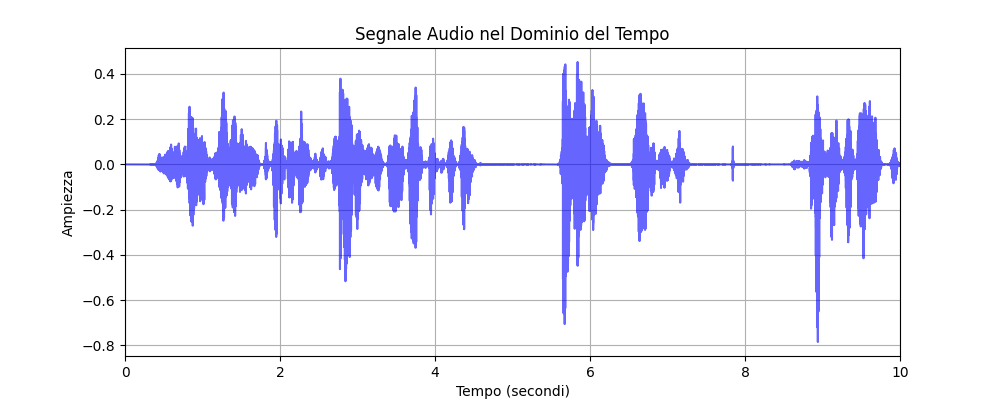
\includegraphics[width=0.8\textwidth]{audio_plot.png}
    \caption{Segnale sinusoidale}
\end{figure}

\subsection{Comunicazione socket}

In questa seconda parte dell'esperienza dobbiamo scrivere uno script python che permetta di inviare e ricevere dati tra due terminali nello stesso pc, per farlo utilizzeremo il pacchetto \textit{socket}. Si andranno a costruire due script:
\begin{itemize}
    \item \textbf{Client:} invia le informazioni;
    \item \textbf{Server:} riceve e processa i dati.
\end{itemize}

Per consentire la comunicazione è necessario creare un "corridoio" tramite il comando \textbf{socket.socket(sk.AF\_INET, sk.SOCK\_STREAM)}, che indica il tipo di indirizzo da utilizzare ed il protocollo di comunicazione (TCP), nel nostro caso \textit{SOCK\_STREAM} garantisce l'invio e la ricezione in ordine dei dati.

Il trasferimento dei dati via socket avviene esclusivamente sotto forma di flusso continuo di \textit{byte}; pertanto, qualsiasi informazione deve essere opportunamente \textbf{codificata} prima dell'invio e \textbf{decodificata} al momento della ricezione. Come primo test, abbiamo realizzato due script per la trasmissione di una semplice stringa di testo.

Cercando di applicare lo stesso metodo ad un array di dati abbiamo riscontrato alcune difficoltà:
\begin{itemize}
    \item utilizzando il comando \textit{dati=sock.recv(1024)} stiamo dicendo di attenderci 1024 bytes di dati, così si rischia di tagliare parte dei dati o includere dati esterni (visto che il socket invia un flusso continuo di dati e l'unico modo per distinguerli e dire esattamente dove inizia e finisce l'informazione)
    \item utilizzando \textit{dati=sock.recv()} il codice riceverà dati finché non sembreranno finiti, per cui il problema sul possibile taglio è risolto, tuttavia abbiamo constatato che per grandi moli di dati, questi possono contenere delle piccole pause che possono far credere al sistema di aver completato la ricezione.
\end{itemize}

Per cui abbiamo scelto di utilizzare un \textit{header}, ovvero un pacchetto di 12 bytes dove sono codificati \textit{samplerate}, \textit{numframes} e la lunghezza in bytes dell'array, così il server all'inizio legge solo quei primi 12 bytes e li decodifica. Ora so esattamente la quantità di dati che mi aspetto, ed essendo potenzialmente di grandi dimensioni abbiamo scelto di riceverli a blocchi (\textit{chunk}) di 4096 che andremo in seguito ad unire per ricostruire l'array inviato, il quale sarà poi riconvertito tramite \textit{np.frombuffer(dati\_completi, dtype=np.float32)}. Stampando il risultato ottenuto ci si accorge che l'array risultante ha una sola dimensione di $960\,000$ elementi ($480\,000 \times 2$). Per ripristinare la matrice stereo originale con forma \texttt{(480000, 2)} necessaria alla riproduzione, abbiamo riorganizzato i due canali separando i campioni in posizione pari e dispari.

Infine, integrando il codice di riproduzione sviluppato nella prima fase, è stato possibile riascoltare correttamente l'audio ricevuto dal server.

\section{Conclusioni}

In conclusione, l'esperienza svolta ha permesso di realizzare con successo uno script Python per l'acquisizione di un segnale audio tramite il microfono del computer. È stato compreso il significato fisico dei campioni numerici ottenuti — rappresentanti le variazioni di pressione acustica rispetto al fondo scala dell'ADC — ed è stata visualizzata l'ampiezza di tali oscillazioni in funzione del tempo. Infine, il segnale è stato riascoltato con successo, verificando anche gli effetti della riproduzione a velocità variabile e della normalizzazione dei dati.

Nella seconda fase dell'esperienza, mediante l'impiego del pacchetto \textit{socket}, abbiamo esteso l'applicazione realizzando un'architettura Client-Server tra due terminali. Il segnale audio registrato dal Client è stato trasmesso via rete al Server, il quale ha provveduto a ricomporre l'array dei dati, visualizzarne il grafico e riprodurne l'audio. Per il corretto funzionamento della trasmissione è stato fondamentale l'utilizzo di una struttura a \textit{header}, indispensabile per indicare la dimensione del messaggio e garantire la ricezione completa e ordinata dell'intero flusso di dati.

\end{document}
